\documentclass[11pt,letterpaper]{article}
\usepackage[T1]{fontenc}
\usepackage[scaled]{helvet}
\renewcommand{\familydefault}{\sfdefault}
\usepackage{amsmath,amssymb}
\usepackage[margin=0.8in,bottom=0.9in]{geometry}
\usepackage[most]{tcolorbox}
\usepackage{tikz}
\usetikzlibrary{calc}
\usepackage{enumitem}
\usepackage{array}
\usepackage{needspace}
\usepackage{fancyhdr}
\usepackage{pifont}

% ---- Palette "F. Bright & Playful" ----
\definecolor{fmtitle}{HTML}{3D2C8D}
\definecolor{fmkey}{HTML}{0096C7}
\definecolor{fmwatch}{HTML}{2BB673}
\definecolor{fmturn}{HTML}{F4A100}
\definecolor{fmmistake}{HTML}{EF476F}
\definecolor{fmnotice}{HTML}{9B5DE5}
\definecolor{fmgray}{HTML}{6B6B6B}

\pagestyle{fancy}
\fancyhf{}
\renewcommand{\headrulewidth}{0pt}
\fancyfoot[C]{\footnotesize\color{fmgray}\textcopyright\ 2026 FangMath. All rights reserved.}
\fancyfoot[R]{\footnotesize\color{fmgray}\thepage}
\setlength{\parindent}{0pt}
\setlength{\parskip}{3pt}

\newcommand{\badge}[1]{\colorbox{fmtitle}{\color{white}\bfseries\small\ #1\ }}
\newcommand{\leveltag}[2]{\colorbox{#1}{\color{white}\bfseries\scriptsize\ #2\ }}
\newcommand{\LE}{\leveltag{fmwatch}{EASY}}
\newcommand{\LM}{\leveltag{fmturn}{MEDIUM}}
\newcommand{\LH}{\leveltag{fmmistake}{HARD}}

\newcommand{\sectionbar}[2]{\needspace{6cm}\par\vspace{4mm}
  \begin{tcolorbox}[enhanced,colback=fmtitle,colframe=fmtitle,arc=2mm,
    left=4mm,top=1.5mm,bottom=1.5mm]
  \color{white}\bfseries\large #1\hfill{\normalsize\mdseries #2}
  \end{tcolorbox}}

\newtcolorbox{keyidea}{enhanced,breakable,colback=white,colframe=fmkey,boxrule=1pt,arc=2mm,
  title={Key Idea},coltitle=fmkey,fonttitle=\bfseries,
  attach boxed title to top left={xshift=4mm,yshift=-2mm},
  boxed title style={colback=white,colframe=fmkey,boxrule=0.9pt}}
\newtcolorbox{watchme}{enhanced,colback=white,colframe=fmwatch,boxrule=1pt,arc=2mm,
  title={Watch Me --- Worked Example},coltitle=fmwatch,fonttitle=\bfseries,
  attach boxed title to top left={xshift=4mm,yshift=-2mm},
  boxed title style={colback=white,colframe=fmwatch,boxrule=0.9pt}}
\newtcolorbox{mistakebox}{enhanced,breakable,colback=white,colframe=fmmistake,boxrule=1pt,arc=2mm,
  title={Common Mistake},coltitle=fmmistake,fonttitle=\bfseries,
  attach boxed title to top left={xshift=4mm,yshift=-2mm},
  boxed title style={colback=white,colframe=fmmistake,boxrule=0.9pt}}
\newtcolorbox{yourturn}{enhanced,breakable,colback=white,colframe=fmturn,boxrule=1pt,arc=2mm,
  title={Your Turn},coltitle=fmturn,fonttitle=\bfseries,
  attach boxed title to top left={xshift=4mm,yshift=-2mm},
  boxed title style={colback=white,colframe=fmturn,boxrule=0.9pt}}
\newtcolorbox{answerbox}[1]{enhanced,breakable,colback=white,colframe=fmwatch,boxrule=1pt,arc=2mm,
  title={#1},coltitle=fmwatch,fonttitle=\bfseries,
  attach boxed title to top left={xshift=4mm,yshift=-2mm},
  boxed title style={colback=white,colframe=fmwatch,boxrule=0.9pt}}

\newcommand{\work}[1]{\par\vspace{#1}}
\setlist[enumerate]{itemsep=2pt,topsep=3pt}

% ---------------- extra boxes ----------------
\newtcolorbox{notebox}{enhanced,breakable,colback=white,colframe=fmnotice,boxrule=1pt,arc=2mm,
  title={Notice},coltitle=fmnotice,fonttitle=\bfseries,
  attach boxed title to top left={xshift=4mm,yshift=-2mm},
  boxed title style={colback=white,colframe=fmnotice,boxrule=0.9pt}}
\newtcolorbox{exbox}{enhanced,colback=white,colframe=fmwatch,boxrule=0.8pt,arc=2mm,
  title={Example},coltitle=fmwatch,fonttitle=\bfseries\small,
  attach boxed title to top left={xshift=4mm,yshift=-2mm},
  boxed title style={colback=white,colframe=fmwatch,boxrule=0.8pt},fontupper=\small}
\newcommand{\topicbar}[1]{\needspace{4.5cm}\par\vspace{5mm}
  \begin{tcolorbox}[enhanced,colback=fmtitle,colframe=fmtitle,arc=2mm,left=4mm,top=1.5mm,bottom=1.5mm]
  \color{white}\bfseries\large #1
  \end{tcolorbox}}
\usepackage{multicol}

% ---------------- practice layout ----------------
\newcommand{\workline}{\par\vspace{7mm}{\color{gray!55}\rule{\linewidth}{0.4pt}}}
\newcommand{\worklines}[1]{\foreach \i in {1,...,#1}{\workline}}
\newcommand{\prob}[3]{\needspace{#3}\par\vspace{3mm}{\color{fmturn}\bfseries #1.}\ #2\par}
\newcommand{\ansline}{\par\vspace{4mm}\hfill\textbf{Answer:}\ \rule{5cm}{0.4pt}\par}
\newcommand{\keyitem}[3]{\needspace{3.2cm}\par\vspace{2mm}
  \begin{tcolorbox}[enhanced,colback=white,colframe=fmwatch!60,boxrule=0.6pt,arc=1.5mm,left=3mm,top=1.5mm,bottom=1.5mm]
  {\color{fmwatch}\bfseries #1.}\quad\small #2\par\vspace{1mm}
  \normalsize\textbf{Answer: #3}
  \end{tcolorbox}}


\usetikzlibrary{arrows.meta}
\providecommand{\iskey}{0}
% fill-in blank: line for students, pink answer in the key
\newcommand{\fb}[2][2.6cm]{\ifnum\iskey=1 \underline{\makebox[#1][c]{\color{fmmistake}\bfseries #2}}\else\underline{\makebox[#1]{}}\fi}
% answer line for practice problems
\newcommand{\pans}[2][3.2cm]{\ifnum\iskey=1 \underline{\makebox[#1][c]{\color{fmmistake}\bfseries #2}}\else\rule{#1}{0.4pt}\fi}
\newcommand{\vid}[1]{{\color{fmgray}\small\textit{\ding{43} Video: #1}}}
\newcommand{\pt}[2]{\fill (#1) circle (2.2pt) node[above=1pt,font=\small]{$#2$};}

\usetikzlibrary{decorations.pathreplacing}
\newcommand{\gridb}[4]{\draw[gray!30,step=1] (#1,#2) grid (#3,#4);\draw[gray!70,-{Stealth}] (#1,0)--(#3+0.4,0);\draw[gray!70,-{Stealth}] (0,#2)--(0,#4+0.4);}
\newcommand{\sdp}[3]{\begin{minipage}[t][2.4cm]{0.48\linewidth}{\color{fmturn}\bfseries #1.}\ #2\par\vfill\hfill \pans[3.6cm]{#3}\end{minipage}}
\newcommand{\sdpw}[3]{\begin{minipage}[t][2.4cm]{0.48\linewidth}{\color{fmturn}\bfseries #1.}\ #2\par\vfill\hfill \pans[5.2cm]{#3}\end{minipage}}
\newcommand{\algp}[3]{\begin{minipage}[t][4.2cm]{0.48\linewidth}{\color{fmturn}\bfseries #1.}\ #2\par\vfill\hfill \pans[4.4cm]{#3}\end{minipage}}
\newcommand{\pair}[2]{\needspace{3.4cm}\noindent #1\hfill #2\par\vspace{2mm}}
\newcommand{\head}[2]{\ifnum\iskey=1 \colorbox{fmwatch}{\color{white}\bfseries\small\ ANSWER KEY\ }\else\badge{#1}\fi\hfill{\small\color{fmgray}Geometry \textperiodcentered\ Lesson #2}\par\vspace{4mm}}
\newcommand{\nameline}{Name: \rule{6cm}{0.4pt}\hspace{1cm}Date: \rule{3.5cm}{0.4pt}\par\vspace{2mm}}
\renewcommand{\vid}[1]{\needspace{4.2cm}{\color{fmgray}\small\textit{\ding{43} Video: #1}}}
\begin{document}
\head{WATCH \& FILL IN}{1.4}
{\color{fmtitle}\LARGE\bfseries Perimeter \& Area in the Coordinate Plane --- Notes\ifnum\iskey=1 \ --- Key\fi}\par\vspace{1mm}
{\color{fmgray}Watch the video and fill in each blank. Pause when you see ``Your turn.''}\par\vspace{3mm}
\nameline

\vid{Side lengths from coordinates}
\begin{keyidea}\begin{minipage}[c]{0.4\linewidth}\centering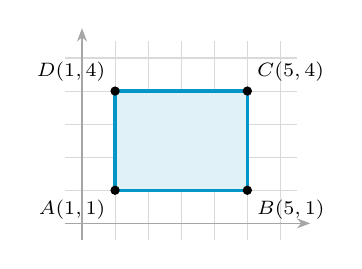
\begin{tikzpicture}[scale=0.42]\gridb{-0.5}{-0.5}{6.5}{5.5}
\draw[very thick,fmkey,fill=fmkey!12] (1,1)--(5,1)--(5,4)--(1,4)--cycle;
\fill (1,1) circle(4pt) node[below left,font=\scriptsize]{$A(1,1)$} (5,1) circle(4pt) node[below right,font=\scriptsize]{$B(5,1)$} (5,4) circle(4pt) node[above right,font=\scriptsize]{$C(5,4)$} (1,4) circle(4pt) node[above left,font=\scriptsize]{$D(1,4)$};\end{tikzpicture}\end{minipage}\hfill
\begin{minipage}[c]{0.56\linewidth}Rectangle $ABCD$:\par\vspace{1mm}
$AB = 5 - 1 = $ \fb[1cm]{$4$} \qquad $BC = 4 - 1 = $ \fb[1cm]{$3$}\par\vspace{2mm}
Same $y$: subtract the \fb[1.2cm]{$x$}'s. \quad Same $x$: subtract the \fb[1.2cm]{$y$}'s.\end{minipage}\end{keyidea}

\vid{Perimeter and area}
\begin{keyidea}\textbf{Perimeter} $=$ \fb[3.4cm]{add all the sides}: \ $P = 4 + 3 + 4 + 3 = $ \fb[1.2cm]{$14$}\par\vspace{2mm}
\textbf{Area} $=$ \fb[3.4cm]{base $\times$ height}: \ $A = 4 \cdot 3 = $ \fb[1.2cm]{$12$}\par\vspace{2mm}
Perimeter is a length: \fb[1.4cm]{units}. \ Area counts squares: \fb[2.6cm]{square units}.\end{keyidea}

\vid{Area of a triangle}
\begin{keyidea}\begin{minipage}[c]{0.4\linewidth}\centering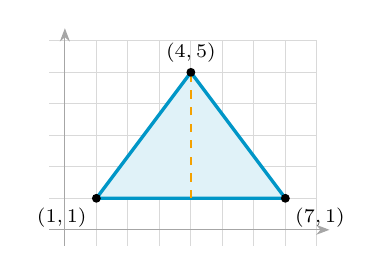
\begin{tikzpicture}[scale=0.4]\gridb{-0.5}{-0.5}{8}{6}
\draw[very thick,fmkey,fill=fmkey!12] (1,1)--(7,1)--(4,5)--cycle;\draw[fmturn,thick,dashed] (4,1)--(4,5);
\fill (1,1) circle(4pt) node[below left,font=\scriptsize]{$(1,1)$} (7,1) circle(4pt) node[below right,font=\scriptsize]{$(7,1)$} (4,5) circle(4pt) node[above,font=\scriptsize]{$(4,5)$};\end{tikzpicture}\end{minipage}\hfill
\begin{minipage}[c]{0.56\linewidth}base $= 7 - 1 = $ \fb[1cm]{$6$}\par\vspace{1mm}
height $= 5 - 1 = $ \fb[1cm]{$4$} \ (straight \fb[1.2cm]{up} from the base)\par\vspace{1mm}
$A = $ \fb[1.4cm]{$\tfrac12$} $\cdot\, b \cdot h = \tfrac12 \cdot 6 \cdot 4 = $ \fb[1.2cm]{$12$}\end{minipage}\end{keyidea}

\vid{A slanted side? Use Pythagoras}
\begin{keyidea}Same triangle. A slanted side goes across $3$ and up $4$: \ $\sqrt{3^2 + 4^2} = \sqrt{25} = $ \fb[1cm]{$5$}.\par\vspace{1mm}
The other slanted side is also $5$. \quad $P = 6 + 5 + 5 = $ \fb[1.2cm]{$16$}\end{keyidea}

\vid{Watch out}
\begin{mistakebox}For a \fb[1.8cm]{slanted} side you can't just count squares. Use the \fb[3.2cm]{Distance Formula} --- or draw the right triangle and use \fb[2.6cm]{Pythagoras}.\end{mistakebox}

\vid{Your turn}
\begin{yourturn}\begin{minipage}[c]{0.66\linewidth}Triangle $P(0,0)$, $Q(6,0)$, $R(0,8)$. Find its perimeter and area.\par\vspace{2mm}
$PQ = 6,\ PR = 8$, \quad $QR = \sqrt{6^2 + 8^2} = $ \fb[1.2cm]{$10$}\par\vspace{1mm}
Perimeter $= 6 + 8 + 10 = $ \fb[1.2cm]{$24$} \qquad Area $= \tfrac12 \cdot 6 \cdot 8 = $ \fb[1.2cm]{$24$}\end{minipage}\hfill
\begin{minipage}[c]{0.3\linewidth}\centering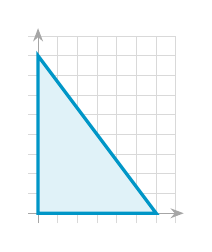
\begin{tikzpicture}[scale=0.25]\gridb{-0.5}{-0.5}{7}{9}
\draw[very thick,fmkey,fill=fmkey!12] (0,0)--(6,0)--(0,8)--cycle;\end{tikzpicture}\end{minipage}\end{yourturn}

\begin{notebox}\textbf{Remember:}\quad Same $y$: subtract the $x$'s; same $x$: subtract the $y$'s.\quad Perimeter: add the sides. Area: rectangle $b \cdot h$, triangle $\tfrac12 bh$.\quad Slanted side: Pythagoras or the Distance Formula.\end{notebox}
\end{document}
